\documentclass[a4paper,11pt]{article}
\usepackage[verbose,a4paper,tmargin=2cm,bmargin=2cm,lmargin=2.5cm,rmargin=2.5cm]{geometry}
\usepackage{polski}
\usepackage{amsmath}
\usepackage{amsfonts}
\usepackage{amssymb}
\usepackage{lastpage}
\usepackage{indentfirst}
\usepackage{verbatim}
\usepackage{graphicx}
\usepackage{fancyhdr}
\usepackage{listings}
\usepackage{float}
\usepackage{hyperref}
\hypersetup{
    colorlinks = true,
    linkcolor = black,
    urlcolor = cyan
}
\usepackage{xcolor}
\usepackage{tikz}
\usepackage{multirow}
\frenchspacing
\pagestyle{fancyplain}
\fancyhf{}

\usepackage{setspace}
\usepackage{enumitem}

\renewcommand{\headrulewidth}{0pt}
\renewcommand{\footrulewidth}{0.4pt}
\newcommand{\degree}{\ensuremath{^{\circ}}} 
\fancyfoot[L]{MUM: P. Galewicz, B. Jurczewski, Z. Nowacki, K.Podlewski, P. Wardęcki}
\fancyfoot[R]{\thepage\ / \pageref{LastPage}}

\begin{document}

%%%%%%%%%%%%%%%%%%%%%%%%%%%%%%%%%%%%%%%%%%%% STRONA TYTUŁOWA

\begin{titlepage}
\begin{center}
\begin{tabular}{rcl}
\begin{tabular}{|r|}
\hline \\
\large{\underline{234053~~~~~~~~~~~~~~~~~~~~~~~} }\\
\small{\textit{Numer indeksu}}\\
\large{\underline{Paweł Galewicz~~~~~~~~~~~~} }\\
\small{\textit{Imię i nazwisko}}\\\\ \hline
\end{tabular} 
&
\begin{tabular}{|r|}
\hline \\
\large{\underline{234067~~~~~~~~~~~~~~~~~~~~~~~} }\\
\small{\textit{Numer indeksu}}\\
\large{\underline{Bartosz Jurczewski~~~~~~~} }\\
\small{\textit{Imię i nazwisko}}\\\\ \hline
\end{tabular} 
&
\begin{tabular}{|r|}
\hline \\
\large{\underline{234102~~~~~~~~~~~~~~~~~~~~~~~} }\\
\small{\textit{Numer indeksu}}\\
\large{\underline{Zbigniew Nowacki~~~~~~~~} }\\
\small{\textit{Imię i nazwisko}}\\\\ \hline
\end{tabular} 
\end{tabular} 

\vspace{10px}

\begin{tabular}{rl}
\begin{tabular}{|r|}
\hline \\
\large{\underline{234106~~~~~~~~~~~~~~~~~~~~~~~} }\\
\small{\textit{Numer indeksu}}\\
\large{\underline{Karol Podlewski~~~~~~~~~~~} }\\
\small{\textit{Imię i nazwisko}}\\\\ \hline
\end{tabular} 
&
\begin{tabular}{|r|}
\hline \\
\large{\underline{234128~~~~~~~~~~~~~~~~~~~~~~~} }\\
\small{\textit{Numer indeksu}}\\
\large{\underline{Piotr Wardęcki~~~~~~~~~~~~} }\\
\small{\textit{Imię i nazwisko}}\\\\ \hline
\end{tabular} 
\end{tabular}
\end{center}

\vspace{25px}

\begin{tabular}{ll}
\LARGE{\textbf{Kierunek}}& \LARGE{Informatyka Stosowana} \\
\LARGE{\textbf{Stopień}}& \LARGE{II} \\
\LARGE{\textbf{Specjalizacja}}& \LARGE{Data Science} \\
\LARGE{\textbf{Semestr}}& \LARGE{1} \\\\
\LARGE{\textbf{Data oddania}}& \LARGE{18 marca 2020} \\\\\\\\\\\\\\
\end{tabular}

\begin{center}
\textbf{\huge{\\~\\Metody uczenia maszynowego }}
\textbf{\Huge{\\~\\Problem set 1}}
\end{center}

\end{titlepage}

\setcounter{page}{2}
\setstretch{1.5}
\tableofcontents
\newpage
\setstretch{1.1}

%%%%%%%%%%%%%%%%%%%%%%%%%%%%%%%%%%%%%%%%%%%% CEL

\section{Cel} \label{sec:cel}
Zadanie polegało na analizie procesu klasyfikacji danych za pomocą wybranych metod:

\begin{enumerate}
    \item Algorytm drzew decyzyjnych
    \item Naiwny klasyfikator Bayesa
    \item Maszyna wektorów nośnych
    \item Klasyfikator k-najbliższych sąsiadów
    \item Algorytm sztucznych sieci neuronowych
\end{enumerate}

Należało zaimplementować każdą metodę, a następnie zweryfikować jej działanie biorąc pod uwagę:

\begin{itemize}
    \item rożne możliwe ustawienia parametrów konfiguracyjnych i ich wpływ na wyniki klasyfikacji
    \item zbiory danych o różnej charakterystyce (przynajmniej 3 różne zbiory)
\end{itemize}

Każdą metodę należało przetestować na tych samych zbiorach, a następnie porównać wyniki i wyciągnąć wnioski dotyczące skuteczności poszczególnych metod. Jako kryterium porównawcze wykorzystaliśmy dokładność klasyfikacji.

%%%%%%%%%%%%%%%%%%%%%%%%%%%%%%%%%%%%%%%%%%%% OPIS IMPLEMENTACJI

\section{Opis implementacji}

Algorytmy zostały zaimplementowane za pomocą języka Python w wersji 3.8.2.
Wykorzystano w nim biblioteki NumPy, Sklearn i Pandas. 

%%%%%%%%%%%%%%%%%%%%%%%%%%%%%%%%%%%%%%%%%%%% OPIS ZBIORÓW DANYCH

\section{Opis zbiorów danych} \label{sec:dataset}

Bazowaliśmy na trzech zestawach danych:

\begin{enumerate}[label=\Alph*.] \label{enum:datasets}
    \item{\href{https://www.kaggle.com/pitasr/falldata}{Fall Detection Data from China}} - zbiór składający się z 6 cech -- czasu oraz pięciu parametrów życiowych. Klasyfikowany jest stan pacjenta w danym przypadku -- stanie, chód, siedzenie, upadek, kurcz, bieg (łącznie 6).
    \item{\href{https://www.kaggle.com/jsphyg/weather-dataset-rattle-package}{Rain in Australia}} -- historia danych pogodowych z 10 lat (data, lokalizacja, temperatury, opady, wiatr, ciśnienie, wilgotność, nasłonecznienie itp). Na podstawie 23 cech należy określić, czy kolejnego dnia wystąpią opady.
    \item{\href{https://www.kaggle.com/uciml/pima-indians-diabetes-database}{Pima Indians Diabetes Database}} -- zbiór danych zawierający 8 niepowiązanych ze sobą pomiarów diagnostycznych (m. in. ilość ciąż, poziom glukozy, ciśnienie, bmi, wiek) na podstawie których dokonywana jest ocena, czy kobieta choruje na cukrzycę.
\end{enumerate}

\section{Klasyfikatory}

\subsection{Algorytm drzew decyzyjnych}
Algorytm polega na stworzeniu modelu do przewidywania wartości na podstawie prostych reguł wywnioskowanych z danych treningowych. Reguły te tworzone są w struktury drzewiaste. Struktury te składają się z:

\begin{itemize}
    \item węzła głównego -- od niego rozpoczyna się proces decyzyjny
    \item węzłów decyzyjnych -- zawierające reguły-zapytania
    \item stanów (liścia) -- końcowych stanów algorytmu, w problemie klasyfikacji są one równoważne z etykietami
    \item połączeń między węzłami -- reprezentującymi możliwe warianty dla danego
\end{itemize}

Zapytania w węzłach są wyrażeniami logicznymi dotyczącymi jednej z cech modelu oraz jej wartości. Wartość ta dobrana musi być w taki sposób, żeby jak najlepiej wydzielić klasę obiektów z przychodzących na węźle danych. Można wtedy powiedzieć, że dany węzeł dostarcza najwięcej informacji. Na potrzebę obliczenia tego przyrostu informacji wprowadza się kryterium \textit{Ipurity}, którego sensem jest fakt, czy po podziale w danym węźle dane zostały poprawnie klasyfikowane. Dokładny sposób wyliczania wartości tego kryterium jest zależny od konfiguracji.
\par
Drzewa domyślnie budowane są do momentu zminimalizowania wartości Impurity, przez co struktura drzew może być bardzo złożona. Skutkiem tego może być przeuczenie modelu, co rzutuje na jego dokładność. Aby ograniczyć możliwość wystąpienia tego zjawiska wprowadza się dodatkowy parametr --  \textit{maksymalna głębokość} -- który mówi o tym ile najwięcej rozgałęzień może wystąpić między węzłem głównym a liściem.

\subsection{Naiwny klasyfikator Bayesa}
Naiwny klasyfikator Bayesa dokonuje klasyfikacji na bazie twierdzenia Bayesa:
$$ P(A \mid B) = \frac{P(B \mid A) \, P(A)}{P(B)} $$
gdzie:
\begin{itemize}
    \item $A$, $B$ -- zdarzenia
    \item $P(A \mid B)$ -- prawdopodobieństwo zdarzenia $A$, o ile zajdzie $B$
    \item $P(B \mid A)$ -- prawdopodobieństwo zdarzenia $B$, o ile zajdzie $A$
    \item $P(A)$ -- prawdopodobieństwo wystąpienia zdarzenia $A$
    \item $P(B)$ -- suma prawdopodobieństw wszystkich potencjalnych skutków zdarzenia: $P(B)=\sum P(B\mid A)P(B)$
\end{itemize}

Model naiwnego klasyfikatora Bayesa zakłada, że dana cecha klasy jest niepowiązana z pozostałymi cechami. Każda z cech indywidualnie wskazuje na prawdopodobieństwo przynależności do danej klasy.
Sprawdza się najlepiej przy dużych zbiorach danych. Jest wykorzystywany m.in. przy filtrowaniu spamu, diagnozie medycznej, czy prognozowaniu pogody.

\subsection{Maszyna wektorów nośnych}
Maszyna wektorów nośnych jest klasyfikatorem liniowym. Algorytm polega na rozdzieleniu obiektów o różnej przynależności klasowej za pomocą hiperpłaszczyzn, które mają być od siebie możliwe jak najbardziej oddalone - taką odległość nazywa się marginesem klasyfikatora, a hiperpłaszczyzny z największym marginesem wektorami nośnymi. 

Algorytm bardzo dobrze sobie radzi z danymi liniowo separowanymi, ale nie zawsze będzie istniała hiperpłaszczyzna rozdzielająca, która zapewni poprawną klasyfikację wszystkich elementów zbioru. W takich przypadkach maszyna wektorów nośnych za pomocą funkcji jądrowych transformuje przestrzeń do postaci liniowo separowanej.

Algorytm umożliwia zmianę wielu parametrów, przy czym najpopularniejsze z nich to:
\begin{itemize}

    \item Regularyzacja - parametr określający jak rygorystyczna jest klasyfikacja. Im większa wartość parametru, tym większy margines ma być znaleziony. Domyślna wartość to 1.
    \item Jądro - typ funkcji przekształcającej problem nierozdzielny do problemu rozdzielnego, na przykład funkcja liniowa, radialna (domyślna), wielomianowa czy sigmoidalna. 
    \item Gamma - określa jak duży wpływ pojedynczy trening ma na inne treningi - im wyższa wartość gammy, tym coraz bardziej podobne muszą być do siebie kolejne próby, by były brane pod uwagę. Ma zastosowanie tylko dla funkcji jądra radialnej, wielomianowej i sigmoidalnej.
\end{itemize}

\subsection{Klasyfikator k-najbliższych sąsiadów}
Algorytm k najbliższych sąsiadów jest klasyfikatorem (ściślej algorytmem regresji regresji nieparametrycznej). Algorytm ten zakłada dany zbiór uczący, w którym znajdują się już sklasyfikowane dane. Schemat składa się z szukania \textit{k} obiektów najbliższych do obiektu klasyfikowanego. Następnie, przyporządkowuje się nowy obiekt do najczęściej występującej klasy w obrębie jego k-najbliższych sąsiadów.

Rysunek \ref{fig:knn} pokazuje działanie algorytmu. W przypadku k=3 (mniejszy okrąg), różowa kropka zostanie zakwalifikowana do niebieskich trójkątów. W przypadku k=5 (większy okrąg) - do pomarańczowych kwadratów.

\begin{figure}[!htbp]
    	\centering
    	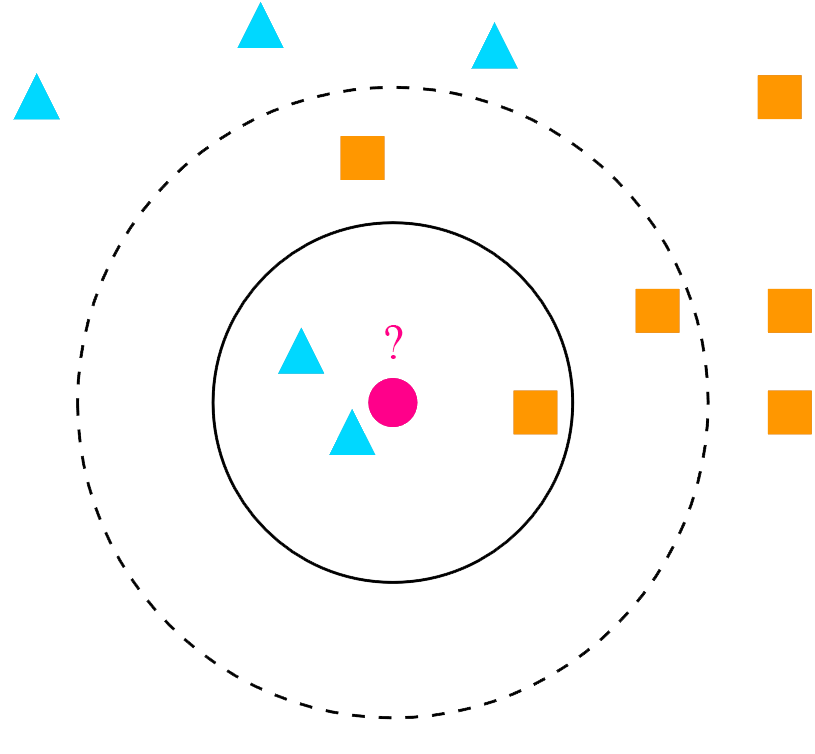
\includegraphics[width=0.45\textwidth]{images/knn.png}
    	\caption{ Wizualizacja klasyfikatora k-najbliższych sąsiadów}
    	\label{fig:knn}
\end{figure}

\subsection{Algorytm sztucznych sieci neuronowych}
Sztuczna siec neuronowa  jest połączeniem wielu elementów nazywanych sztucznymi neuronami, które tworzą co najmniej trzy warstwy: wejściową, ukrytą oraz wyjściową. Neurony przetwarzają informacje dzięki nadaniu im parametrów które nazywane są wagami. Podstawą tworzenia sieci neuronowej jest modyfikowanie współczynnika wagowego połączeń w celu uzyskania poprawnych wyników. W programie użyty został algorytm MLP (ang. Multilayer Perceptron).

%%%%%%%%%%%%%%%%%%%%%%%%%%%%%%%%%%%%%%%%%%%% BADANIA

\section{Badania}

W sekcji badań odnoszono się do zbiorów danych za pomocą oznaczeń zgodnych z sekcją \ref{sec:dataset}.

\subsection{Algorytm drzew decyzyjnych}

\subsubsection*{Wielkość zbioru treningowego}

Na początku sprawdzono wpływ podziału zbioru na części treningowe oraz testowe przy domyślnych cechach klasyfikatora.

\begin{table}[H]
    \centering
    \begin{tabular}{|c|c|c|c|}
    \hline
    \multirow{2}{*}{\textbf{\begin{tabular}[c]{@{}c@{}}\% danych\\ treningowych\end{tabular}}} & \multicolumn{3}{c|}{\textbf{Zbiór danych}} \\ \cline{2-4} 
                                            & \textbf{A}          & \textbf{B}        & \textbf{C}         \\ \hline
    60                                      & 0.678      & 1.0      & 0.668     \\ \hline
    65                                      & 0.681      & 1.0      & 0.717     \\ \hline
    70                                      & 0.677      & 1.0      & 0.711     \\ \hline
    75                                      & 0.687      & 1.0      & 0.739     \\ \hline
    80                                      & 0.693      & 1.0      & 0.680     \\ \hline
    85                                      & 0.697      & 1.0      & 0.703     \\ \hline
    90                                      & 0.690      & 1.0      & 0.699     \\ \hline
    \end{tabular}
    \caption{Porównanie dokładności dla różnych zbiorów, dla drzew decyzyjnych}
    \label{tab:cls1tab1}
\end{table}

Dla 75\% danych testowych dokładność klasyfikacji była nieznacznie lepsza, jednak podział nie miał znaczącego wpływu na ogólne wyniki. Wspomniany podział został wykorzystany przy kolejnych badaniach.

\subsubsection*{Zmiana kryterium Impurity}
Kolejnym badaniem było porównanie wpływu kryterium Impurity, które wykorzystywane jest przy oblicaniu przyrostu informacji.

\begin{table}[H]
    \centering
    \begin{tabular}{|c|c|c|}
    \hline
          & \textbf{Gini}  & \textbf{Entropy} \\ \hline
    Dataset A & 0.696 & 0.711   \\ \hline
    Dataset B & 1.0   & 1.0     \\ \hline
    Dataset C & 0.692 & 0.691   \\ \hline
    \end{tabular}
    \caption{Porównanie dokładności dla różnych kryteriów Impurity algorytmu drzew decyzyjnych}
    \label{tab:cls1tab2}
\end{table}

\subsubsection*{Zmiana maksymalnej głębokości}
Następnie sprawdzono wpływ maksymalnej głębokości. Ustawienie jej może ograniczyć zjawisko przeuczenia się modelu.

\begin{table}[H]
    \centering
    \begin{tabular}{|c|c|c|c|}
    \hline
    \multirow{2}{*}{\textbf{\begin{tabular}[c]{@{}c@{}}Maksymalna\\ głębokość\end{tabular}}} & \multicolumn{3}{c|}{\textbf{Zbiór danych}} \\ \cline{2-4} 
                                                   & \textbf{A}   & \textbf{B}   & \textbf{C}   \\ \hline
    2                                              & 0.363        & 1.0          & 0.710        \\ \hline
    4                                              & 0.408        & 1.0          & 0.721        \\ \hline
    6                                              & 0.477        & 1.0          & 0.735        \\ \hline
    8                                              & 0.565        & 1.0          & 0.712        \\ \hline
    10                                             & 0.640        & 1.0          & 0.705        \\ \hline
    12                                             & 0.674        & 1.0          & 0.697        \\ \hline
    14                                             & 0.683        & 1.0          & 0.699        \\ \hline
    16                                             & 0.691        & 1.0          & 0.711        \\ \hline
    18                                             & 0.693        & 1.0          & 0.696        \\ \hline
    \end{tabular}
    \caption{Porównanie dokładności dla różnej maksymalnej głębokości algorytmu drzew decyzyjnych}
    \label{tab:cls1tab3}
\end{table}

\subsubsection*{Zmiana maksymalnej liczby liści}
Ostatnim eksperymentem było sprawdzenie zależności między maksymalną liczbą liści drzewa, a dokładnością klasyfikacji. Założono, że minimalna liczba liści musi być równa liczbie klas zestawu danych, następnie liczbę tę zwiększano o wielokrotność tej liczby.
\begin{table}[H]
    \centering
    \begin{tabular}{|c|c|c|c|}
    \hline
    \multirow{2}{*}{\textbf{\begin{tabular}[c]{@{}c@{}}Maksymalna\\ liczba liści\end{tabular}}} & \multicolumn{3}{c|}{\textbf{Zbiór danych}} \\ \cline{2-4} 
                                                      & \textbf{A}   & \textbf{B}   & \textbf{C}   \\ \hline
    1x liczba klas                                    & 0.378        & 1.0          & 0.705        \\ \hline
    2x liczba klas                                    & 0.413        & 1.0          & 0.727        \\ \hline
    4x liczba klas                                    & 0.464        & 1.0          & 0.738        \\ \hline
    6x liczba klas                                    & 0.506        & 1.0          & 0.736        \\ \hline
    8x liczba klas                                    & 0.534        & 1.0          & 0.739        \\ \hline
    10x liczba klas                                   & 0.566        & 1.0          & 0.727        \\ \hline
    \end{tabular}
    \caption{Porównanie dokładności dla maksymalnej liczby liści drzewa decyzyjnego}
    \label{tab:cls1tab4}
\end{table}

\subsection{Naiwny klasyfikator Bayesa}
    Przy klasyfikatorze Bayesa nie mamy do dyspozycji parametrów innych niż podział na dane treningowe i testowe. Dokładność klasyfikacji sprawdzono dla każdego ze zbiorów danych w zależności od podziału.

    \begin{table}[H]
        \centering
        \begin{tabular}{|c|c|c|c|}
        \hline
        \multirow{2}{*}{\textbf{\begin{tabular}[c]{@{}c@{}}\% danych\\ treningowych\end{tabular}}} & \multicolumn{3}{c|}{\textbf{Zbiór danych}} \\ \cline{2-4} 
                & \textbf{A}      & \textbf{B}     & \textbf{C}     \\ \hline
        60 \%   & 0.131           & 0.940          & 0.739          \\ \hline
        65 \%   & 0.139           & 0.941          & 0.761          \\ \hline
        70 \%   & 0.132           & 0.942          & 0.761          \\ \hline
        75 \%   & 0.135           & 0.941          & 0.775          \\ \hline
        80 \%   & 0.134           & 0.942          & 0.712          \\ \hline
        85 \%   & 0.138           & 0.939          & 0.730          \\ \hline
        90 \%   & 0.135           & 0.946          & 0.737          \\ \hline
        \end{tabular}
        \caption{Porównanie dokładności dla różnych zbiorów, dla naiwnego klasyfikatora Bayesa}
        \label{tab:cls2tab1}
    \end{table}
    
    Dokładność klasyfikacji zależy przede wszystkim od samego zbioru danych. Natomiast jego podział ma pomijalny wpływ na wyniki.

\subsection{Maszyna wektorów nośnych}

\subsubsection*{Wielkość zbioru treningowego}

Na początku sprawdzono wpływ podziału zbioru na części treningowe oraz testowe przy domyślnych cechach klasyfikatora.

\begin{table}[H]
    \centering
    \begin{tabular}{|c|c|c|c|}
    \hline
    \multirow{2}{*}{\textbf{\begin{tabular}[c]{@{}c@{}}\% danych\\ treningowych\end{tabular}}} & \multicolumn{3}{c|}{\textbf{Zbiór danych}} \\ \cline{2-4} 
            & \textbf{A}      & \textbf{B}     & \textbf{C}     \\ \hline
    60 \%   & 0.3             & 0.803          & 0.762          \\ \hline
    65 \%   & 0.317           & 0.809          & 0.761          \\ \hline
    70 \%   & 0.326           & 0.813          & 0.757          \\ \hline
    75 \%   & 0.341           & 0.818          & 0.78           \\ \hline
    80 \%   & 0.33            & 0.818          & 0.725          \\ \hline
    85 \%   & 0.322           & 0.817          & 0.73           \\ \hline
    90 \%   & 0.324           & 0.819          & 0.737          \\ \hline
    \end{tabular}
    \caption{Porównanie dokładności dla różnych zbiorów, dla maszyny wektorów nośnych}
    \label{tab:cls3tab1}
\end{table}

Podział zbioru nie wpływa w znaczącym stopniu na dokładność klasyfikacji. Średnio najlepsze wyniki uzyskano dla zbioru treningowego stanowiącego 75\%, i to właśnie taki podział będzie stosowany przy analizie wpływu zmiany parametrów klasyfikatora. 

\subsubsection*{Zmiana parametru regularyzacji oraz funkcji jądra}

Następnie porównano wpływ zmiany parametru regularyzacji oraz funkcji jądra na uzyskane wyniki.

Liniowa funkcja jądra nie była w stanie w ciągu 10 minut przeprowadzić klasyfikacji zbioru A, dlatego nie została ona uwzględniona w wynikach. 

\begin{table}[H]
    \centering
    \begin{tabular}{|c|c|c|c|c|}
    \hline
    \multirow{2}{*}{\textbf{\begin{tabular}[c]{@{}c@{}}Parametr\\ regularyzacji\end{tabular}}} & \multicolumn{4}{c|}{\textbf{Funkcja jądrowa}} \\ \cline{2-5} 
        & \textbf{Liniowa} & \textbf{Radialna} & \textbf{Wielomianowa} & \multicolumn{1}{l|}{\textbf{Sigmoidalna}} \\ \hline
    0.1 & -                & 0.286             & 0.275                 & 0.211                                     \\ \hline
    0.2 & -                & 0.294             & 0.271                 & 0.259                                     \\ \hline
    0.5 & -                & 0.293             & 0.292                 & 0.261                                     \\ \hline
    1   & -                & 0.324             & 0.295                 & 0.286                                     \\ \hline
    2   & -                & 0.353             & 0.29                  & 0.277                                     \\ \hline
    5   & -                & 0.393             & 0.294                 & 0.257                                     \\ \hline
    \end{tabular}
    \caption{Porównanie dokładności dla zbioru A przy zmianie regularyzacji oraz funkcji jądra}
    \label{tab:cls3tab2}
\end{table}

\begin{table}[H]
    \centering
    \begin{tabular}{|c|c|c|c|c|}
    \hline
    \multirow{2}{*}{\textbf{\begin{tabular}[c]{@{}c@{}}Parametr\\ regularyzacji\end{tabular}}} & \multicolumn{4}{c|}{\textbf{Funkcja jądrowa}} \\ \cline{2-5} 
        & \textbf{Liniowa} & \textbf{Radialna} & \textbf{Wielomianowa} & \multicolumn{1}{l|}{\textbf{Sigmoidalna}} \\ \hline
    0.1 & 1.0              & 0.784             & 0.779                 & 0.658                                     \\ \hline
    0.2 & 1.0              & 0.774             & 0.788                 & 0.655                                     \\ \hline
    0.5 & 1.0              & 0.786             & 0.807                 & 0.649                                     \\ \hline
    1   & 1.0              & 0.816             & 0.826                 & 0.654                                     \\ \hline
    2   & 1.0              & 0.85              & 0.846                 & 0.654                                     \\ \hline
    5   & 1.0              & 0.87              & 0.88                  & 0.668                                     \\ \hline  
    \end{tabular}
    \caption{Porównanie dokładności dla zbioru B przy zmianie regularyzacji oraz funkcji jądra}
    \label{tab:cls3tab3}
\end{table}

\begin{table}[H]
    \centering
    \begin{tabular}{|c|c|c|c|c|}
    \hline
    \multirow{2}{*}{\textbf{\begin{tabular}[c]{@{}c@{}}Parametr\\ regularyzacji\end{tabular}}} & \multicolumn{4}{c|}{\textbf{Funkcja jądrowa}} \\ \cline{2-5} 
        & \textbf{Liniowa} & \textbf{Radialna} & \textbf{Wielomianowa} & \multicolumn{1}{l|}{\textbf{Sigmoidalna}} \\ \hline
    0.1 & 0.832            & 0.702             & 0.791                 & 0.654                                     \\ \hline
    0.2 & 0.733            & 0.681             & 0.733                 & 0.675                                     \\ \hline
    0.5 & 0.801            & 0.738             & 0.801                 & 0.455                                     \\ \hline
    1   & 0.759            & 0.791             & 0.728                 & 0.545                                     \\ \hline
    2   & 0.796            & 0.696             & 0.738                 & 0.487                                     \\ \hline
    5   & 0.77             & 0.702             & 0.785                 & 0.712                                     \\ \hline
    \end{tabular}
    \caption{Porównanie dokładności dla zbioru C przy zmianie regularyzacji oraz funkcji jądra}
    \label{tab:cls3tab4}
\end{table}

\subsubsection*{Zmiana gammy}

Na sam koniec porównano zmianę gammy dla funkcji radialnej  na zbiorze danych C dla parametru regularyzacji równego 1, mając na celu sprawdzenie, czy dzięki temu będą ona mogła się zbliżyć do dokładności klasyfikacji osiągniętych przez funkcję liniową czy wielomianową.

\begin{table}[H]
    \centering
    \begin{tabular}{|c|c|}
    \hline
    \textbf{Parametr gammy} & \textbf{Funkcja radialna} \\ \hline
    0.1                     & 0.654                     \\ \hline
    0.2                     & 0.634                     \\ \hline
    0.5                     & 0.649                     \\ \hline
    1                       & 0.67                      \\ \hline
    2                       & 0.702                     \\ \hline
    5                       & 0.654                     \\ \hline
    \end{tabular}
    \caption{Porównanie dokładności dla zbioru C przy zmianie gammy dla funkcji jądrowej radialnej}
    \label{tab:cls3tab5}
\end{table}


\subsection{Klasyfikator k-najbliższych sąsiadów}

Na początku sprawdzono wpływ podziału zbioru na części treningowe oraz testowe przy domyślnych cechach klasyfikatora.

\begin{table}[H]
    \centering
    \begin{tabular}{|c|c|c|c|}
    \hline
    \multirow{2}{*}{\textbf{\begin{tabular}[c]{@{}c@{}}\% danych \\ treningowych\end{tabular}}} & \multicolumn{3}{c|}{\textbf{Zbiór danych}} \\ \cline{2-4} 
     & \textbf{A} & \textbf{B} & \textbf{C} \\ \hline
    60\% & 0.638 & 0.858 & 0.713 \\ \hline
    65\% & 0.646 & 0.862 & 0.664 \\ \hline
    70\% & 0.65 & 0.859 & 0.752 \\ \hline
    75\% & 0.651 & 0.866 & 0.738 \\ \hline
    80\% & 0.652 & 0.859 & 0.719 \\ \hline
    85\% & 0.644 & 0.872 & 0.722 \\ \hline
    90\% & 0.668 & 0.859 & 0.658 \\ \hline
    \end{tabular}
    \caption{Porównanie dokładności dla różnych zbiorów, dla klasyfikatora k-najbliższych sąsiadów}
    \label{tab:cls4tab1}
\end{table}

Podział zbioru nie wpływa w znaczącym stopniu na dokładność klasyfikacji. Średnio najlepsze wyniki uzyskano dla zbioru treningowego stanowiącego 85\%, i to właśnie taki podział będzie stosowany przy analizie wpływu zmiany parametrów klasyfikatora. 

\begin{table}[H]
    \centering
    \begin{tabular}{|c|c|c|c|}
    \hline
    \multirow{2}{*}{\textbf{Liczba sąsiadów}} & \multicolumn{3}{c|}{\textbf{Zbiór danych}} \\ \cline{2-4} 
     & \textbf{A} & \textbf{B} & \textbf{C} \\ \hline
    2 & 0.669 & 0.853 & 0.713 \\ \hline
    3 & 0.670 & 0.857 & 0.678 \\ \hline
    4 & 0.670 & 0.859 & 0.687 \\ \hline
    5 & 0.659 & 0.868 & 0.791 \\ \hline
    6 & 0.656 & 0.866 & 0.774 \\ \hline
    \end{tabular}
    \caption{Porównanie dokładności dla różnych zbiorów klasyfikatora k-najbliższych sąsiadów, przy zmianie liczby sąsiadów}
    \label{tab:cls4tab2}
\end{table}

\subsection{Algorytm sztucznych sieci neuronowych}
Dla poszczególnych zbiorów danych najlepsze wyniki uzyskano dla 70 \% danych treningowych. Następnie przystąpiono do badania wpływu zmian parametrów na klasyfikator. W tym celu zmieniana była liczba warstw ukrytych w algorytmie.
\begin{table}[H]
    \centering
    \begin{tabular}{|c|c|c|c|}
    \hline
    \multirow{2}{*}{\textbf{\begin{tabular}[c]{@{}c@{}}\% danych\\ treningowych\end{tabular}}} & \multicolumn{3}{c|}{\textbf{Zbiór danych}} \\ \cline{2-4} 
            & \textbf{A}      & \textbf{B}     & \textbf{C}     \\ \hline
    60 \%   & 0.281             & 0.997          & 0.664          \\ \hline
    65 \%   & 0.284           & 0.990          & 0.683          \\ \hline
    70 \%   & 0.285           & 0.993          & 0.700          \\ \hline
    75 \%   & 0.275           & 0.992          & 0.665           \\ \hline
    80 \%   & 0.281            & 0.965          & 0.693          \\ \hline
    85 \%   & 0.278           & 0.988          & 0.617           \\ \hline
    90 \%   & 0.280           & 0.994          & 0.684          \\ \hline
    \end{tabular}
    \caption{Porównanie dokładności dla różnych zbiorów, dla sztucznych sieci neuronowych}
    \label{tab:cls5tab1}
\end{table}

\begin{table}[H]
    \centering
    \begin{tabular}{|c|c|c|c|}
    \hline
    \multirow{2}{*}{\textbf{\begin{tabular}[c]{@{}c@{}}Liczba\\
    warstw ukrytych\end{tabular}}} & \multicolumn{3}{c|}{\textbf{Zbiór danych}} \\ \cline{2-4} 
            & \textbf{A}      & \textbf{B}     & \textbf{C}     \\ \hline
    50    & 0.232             & 0.882         & 0.691          \\ \hline
    100   & 0.285           & 0.993          & 0.700          \\ \hline
    200   & 0.275           & 0.983          & 0.730          \\ \hline
    300   & 0.287           & 0.782          & 0.652           \\ \hline
    400   & 0.285            & 0.995          & 0.713          \\ \hline
    500   & 0.288           & 0.978          & 0.717           \\ \hline
    \end{tabular}
    \caption{Porównanie dokładności dla różnych zbiorów, dla 70 \% danych treningowych oraz różnej liczby warstw ukrytych}
    \label{tab:cls5tab2}
\end{table}




%%%%%%%%%%%%%%%%%%%%%%%%%%%%%%%%%%%%%%%%%%%% WNIOSKI

\section{Wnioski}

\subsection*{Drzewa decyzyjne}
\begin{itemize}
    \item Zbiór danych mówiący o deszczach nie był dobrze dobrany do wykonywania testów tego algorytmu.
    \item Oba rodzaje kryterium Impurity dostarczały podobnych rezultatów.
    \item Do poprawnej klasyfikacji wymagana jest odpowiednio dobrana do zestawu danych maksymalna głębokość. Jak widać w tabeli \ref{tab:cls1tab3}, dla zbioru o wielu klasach jest ona zdecydowanie większa niż dla zbioru z dwoma klasami. Dla zbioru C zauważalny jest efekt przeuczenia.
    \item Podobnie jest w przypadku liczby liści, przy czym ich liczba równa liczbie klas zbioru okazuje się być zdecydowanie za mała.
\end{itemize}

\subsection*{Naiwny klasyfikator Bayesa}
\begin{itemize}
    \item Większa liczba cech, a mniejsza klas pozwala na dokładniejszą klasyfikację
    \item Rozmiar zbioru treningowego ma pomijalny wpływ na dokładność klasyfikacji
\end{itemize}

\subsection*{Maszyna wektorów nośnych}
\begin{itemize}
    \item Maszyna wektorów nośnych nie radzi sobie dobrze z klasyfikacją zbioru danych dotyczącego upadków ludzi w chinach (zbiór A) - jest to prawdopodobnie spowodowane większą liczbą klas do odróżnienia, kiedy algorytm najlepiej sobie radzi przy dwóch klasach. Zbiór ten był najdłuższej oraz najgorzej klasyfikowany.
    \item Parametr regularyzacji najlepiej się sprawdzał, kiedy jego wartość oscylowała w pobliżu wartości domyślnej równej 1.
    \item Najlepszą funkcją jadra przy klasyfikacji zbiorów opisanych w sekcji \ref{sec:dataset} okazała się funkcja liniowa. Bardzo dobre wyniki osiągały też funkcje radialna oraz wielomianowa. Dla sprawdzanych zbiorów danych zdecydowanie najgorsza okazała się funkcja sigmoidalna.
    \item Zmiana gammy nie wpłynęła zauważalnie na wyniki klasyfikacji na zbiorze dotyczącym cukrzyków. 
\end{itemize}

\subsection*{Klasyfikator k-najbliższych sąsiadów}
\begin{itemize}
    \item Klasyfikator najlepsze wyniki osiąga na dużych zbiorach danych (zbiór B) w których to dane są ze sobą mocno skorelowane.
    \item Zmiana liczby sąsiadów nie miała dużego przełożenia na współczynnik
    dokładności.
\end{itemize}

\subsection*{Sztuczna sieć neuronowa}
\begin{itemize}
    \item Sztuczna sieć neuronowa najlepsze wyniki osiąga na dużych zbiorach danych (zbiór B) w których to dane są ze sobą mocno skorelowane.
    \item Średnio najlepsze wyniki dla wszystkich zbiorów danych uzyskiwane były dla 400 warstw ukrytych
\end{itemize}

\end{document}
